%iffalse
\let\negmedspace\undefined
\let\negthickspace\undefined
\documentclass[journal,12pt,twocolumn]{IEEEtran}
\usepackage{cite}
\usepackage{amsmath,amssymb,amsfonts,amsthm}
\usepackage{algorithmic}
\usepackage{graphicx}
\usepackage{textcomp}
\usepackage{xcolor}
\usepackage{txfonts}
\usepackage{listings}
\usepackage{enumitem}
\usepackage{mathtools}
\usepackage{gensymb}
\usepackage{comment}
\usepackage[breaklinks=true]{hyperref}
\usepackage{tkz-euclide} 
\usepackage{listings}
\usepackage{gvv}                                        
\def\inputGnumericTable{}                                 
\usepackage[latin1]{inputenc}                                
\usepackage{color}                                            
\usepackage{array}                                            
\usepackage{longtable}                                       
\usepackage{calc}                                             
\usepackage{multirow}                                         
\usepackage{hhline}                                           
\usepackage{ifthen}                                           
\usepackage{lscape}

\newtheorem{theorem}{Theorem}[section]
\newtheorem{problem}{Problem}
\newtheorem{proposition}{Proposition}[section]
\newtheorem{lemma}{Lemma}[section]
\newtheorem{corollary}[theorem]{Corollary}
\newtheorem{example}{Example}[section]
\newtheorem{definition}[problem]{Definition}
\newcommand{\BEQA}{\begin{eqnarray}}
\newcommand{\EEQA}{\end{eqnarray}}
\newcommand{\define}{\stackrel{\triangle}{=}}
\theoremstyle{remark}
\newtheorem{rem}{Remark}
\begin{document}

\bibliographystyle{IEEEtran}
\vspace{3cm}

\title{10.5.2.7}
\author{EE23BTECH11017 - Eachempati Mihir Divyansh$^{*}$% <-this % stops a space
}
\maketitle
\newpage
\bigskip

\renewcommand{\thefigure}{\theenumi}
\renewcommand{\thetable}{\theenumi}

\textbf{Question:} Find the 31st term of an AP whose $11$th term is 38 and the $16$th term is 73.
\\
\solution
% \fi
\\

\begin{table}[h]
    \centering
    \caption{Given Values}
    \begin{tabular}{|m{2cm}|m{2cm}|m{2cm}|}
    \hline
    \textbf{Symbol} & \textbf{Value} & \textbf{Description}\\ [1ex]
    \hline
        $x$ & $x\brak{0}r^4$ & $x\brak{4}$ \\ [1ex]
    \hline
        $y$ & $x\brak{0}r^{10}$ & $x\brak{10}$\\ [1ex]
    \hline
        $z$ & $x\brak{0}r^{16}$ & $x\brak{16}$\\ [1ex]
    \hline
        $r$ & ? & $\frac{x\brak{n}}{x\brak{n-1}}$\\[1ex]
    \hline \vspace{0.1cm}
        $x\brak{0}$ & ? & First term \\[1ex]
    \hline
        $x\brak{n}$ & $x\brak{0}r^nu\brak{n}$ & General Term \\ [1ex]
    \hline
    \end{tabular}
\label{tab:1}
\end{table}
From Table 
\begin{align}
x\brak{0}+10d&=38\label{10.5.2.7.eq: 1}\\
x\brak{0}+15d&=73 \label{10.5.2.7.eq: 2}
\end{align}
From  equations \ref{10.5.2.7.eq: 1} and \ref{10.5.2.7.eq: 2}, the augmented matrix is:
\begin{align}
 \myvec{
   1 & 10 & 38
   \\
   1 & 15 & 73
 } 
 \xleftrightarrow[]{R_2 \rightarrow R_2-R_1} 
  \myvec{
   1 & 10 & 38
   \\
   0 & 5 & 35
 } \\
 \xleftrightarrow[]{R_1 \rightarrow R_1-2R_2} 
  \myvec{
   1 & 0 & -32
   \\
   0 & 5 & 35
 } \\
  \xleftrightarrow[]{R_2 \rightarrow \frac{R_2}{5}} 
  \myvec{
   1 & 0 & -32
   \\
   0 & 1 & 7
 } \\
 \implies \myvec{
   x\brak{0}
   \\
   d
 }
 =
 \myvec{
   -32
   \\
   7
 }
 \end{align}
 The general term and the Z-transform are given by

 \begin{align}
    x\brak{n}&=\brak{-32+7n}u\brak{n}\\ 
 \end{align}

The 31st term of this A.P. is 
\begin{align}x\brak{30}&=178\end{align}
 From \eqref{eq:APSum}, the Z-Transform of $x\brak{n}$ is given by 
\begin{align}
    X\brak{z}&=\frac{-32}{1-z^{-1}}+\frac{7z^{-1}}{\brak{1-z^{-1}}^2}
\end{align}
 \begin{figure}[h]
    \centering
    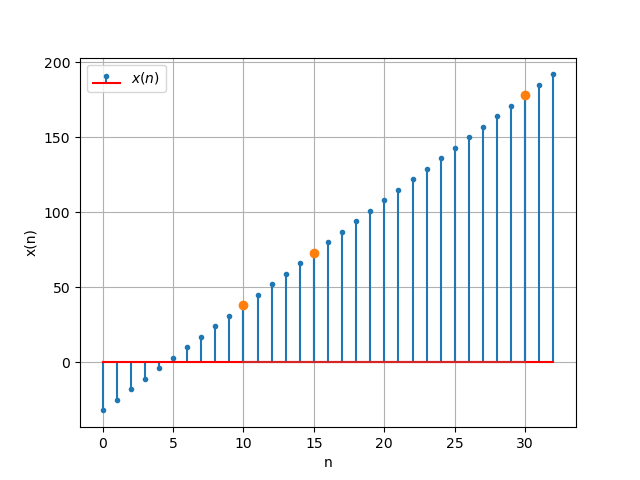
\includegraphics[width=\columnwidth]{figs/fig1.png}
    \caption{Stem plot of $x(0)$ v/s $n$}
 \end{figure}

\end{document}
